\documentclass[a4paper]{article}
\title{Radial Electric Field-Generating Terms in L-H Transitions}
\author{{\Large Kevin A. Blondino} \\
	Supervisor: dr. H.J. de Blank \\
	\textsc{Eindhoven University of Technology} \\
	\texttt{k.blondino@student.tue.nl}}
\date{14 August 2017}

%{{{ Packages
\usepackage{fullpage,amsmath,graphicx,indentfirst}
\usepackage[labelfont=bf]{caption}

\usepackage{cleveref}

\usepackage{lipsum,xcolor}
\newcommand\mynotes[1]{\textcolor{red}{#1}}
%}}}

\linespread{1.1}

%{{{ Setup References
\usepackage[backend=bibtex,url=false]{biblatex}
\addbibresource{../../References/References.bib}
%}}}

\usepackage{hyperref}
\hypersetup
{
	pdfauthor={Kevin A. Blondino}
	pdftitle={$E_r$-Generating Terms}
	pdfsubject={Radial Electric Field-Generating Terms in L-H Transitions}
	pdfkeywords={Prelude, H-mode, L-mode, bifurcation}
}


%{{{ Two Figures Side-by-Side
\newsavebox\IBoxA \newsavebox\IBoxB \newlength\IHeight
\newcommand\TwoFig[6]{% Image1 Caption1 Label1 Im2 Cap2 Lab2
	\sbox\IBoxA{\includegraphics[width=0.45\textwidth]{#1}}
	\sbox\IBoxB{\includegraphics[width=0.45\textwidth]{#4}}%
	\ifdim\ht\IBoxA>\ht\IBoxB
		\setlength\IHeight{\ht\IBoxB}%
	\else\setlength\IHeight{\ht\IBoxA}\fi
	\begin{figure}[tb]
		\minipage[t]{0.45\textwidth}\centering
			\includegraphics[height=\IHeight]{#1}
			\caption{#2}\label{#3}
		\endminipage\hfill
		\minipage[t]{0.45\textwidth}\centering
			\includegraphics[height=\IHeight]{#4}
			\caption{#5}\label{#6}
		\endminipage
	\end{figure}%
}
%}}}

%--------------------------------------

\begin{document}
\maketitle

%--------------------------------------

\begin{abstract}
	
The viability of tokamaks as a energy source relies on its operation mode, as anomalous transport dominates confinement.
H--mode is defined as a reduction in this transport; there does not yet exist a comprehensive theory of the fundamental physics of this mode and the L--H transition.
What is established is that a radial electric field at the plasma edge is known to be an integral part in the processes of this operational mode.

The topic of this study is determine the dominance of mechanisms that generate this radial electric field.
A mathematical model is used to simulate the dynamics near the edge of the plasma, with many of the effects in generating and suppressing the field as additive terms in an equation for a radial displacement current.
The forms of these mechanisms can greatly affect the underlying mathematical behavior.

The dynamics of the system generated both expected and unexpected results.
An operational mode somewhat resembling H--mode was formed when supplied by adequate input power.
One nonambipolar flux was found to dominate: the ion bulk viscosity.
However, unphysical oscillations and occasional lack of a steady-state were found in the system, with no current explanation.
The forms of the mechanisms therefore require more scrutiny.


\end{abstract}

\section{Introduction and Background}
\subsection{H-mode}
\begin{figure}[b]
\begin{minipage}{0.48\linewidth}
	\centering
	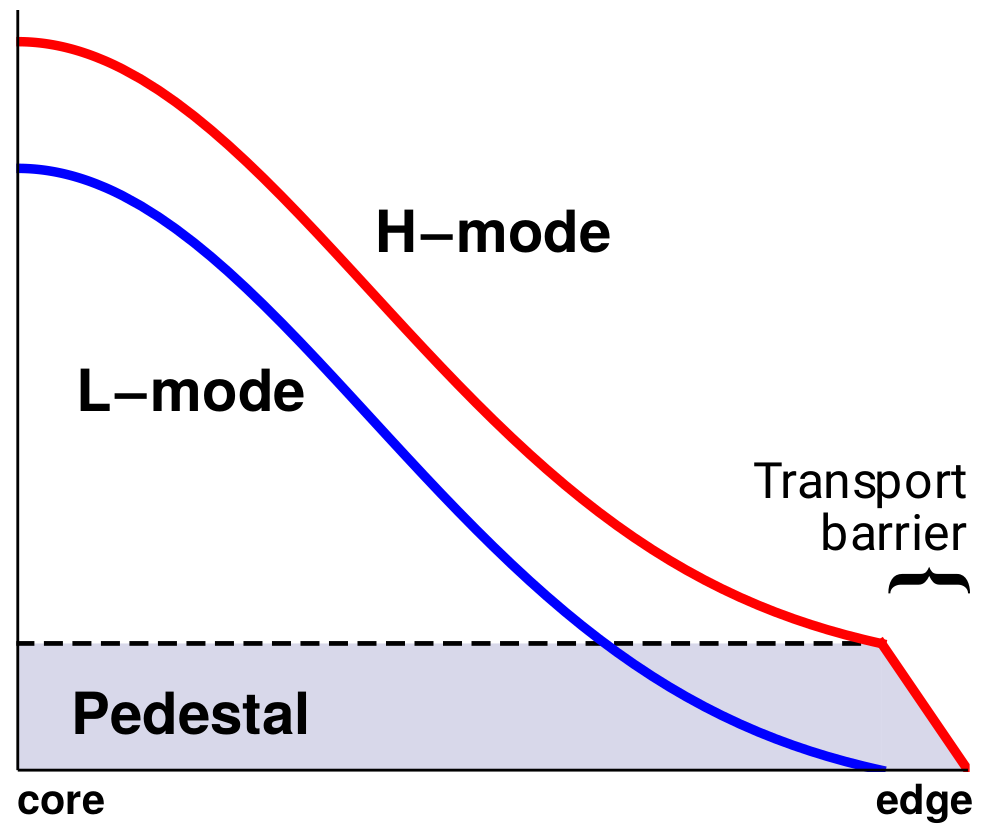
\includegraphics[width=0.8\textwidth]{../../Graphics/L-mode_H-mode_compare.png}
\end{minipage}
\hfill
\begin{minipage}{0.48\linewidth}
	\caption{A comparison of the radial pressure profiles of L-mode and H-mode.
	The profile of H-mode can be thought of as on a `pedestal,' in which the pressure profile is increase in the core.
	This is due to the transport barrier that is formed at the edge \cite{weymiens_bifurcation_2014}.}
	\label{fig:L-mode_H-mode_compare}
\end{minipage}
\end{figure}

In 1982, a new NBI system was install in the ASDEX tokamak, which pushed it into a new realm.
A new level of energy confinement time was achieved, measured to be a factor of 2 or more than previous.
This state of operation was coined the high-confinement (H-) mode, and is now considered necessary for the future of nuclear fusion as an energy source \cite{arnoux_how_2009} \cite{wagner_development_1984}.

Transport of particles and energy in tokamaks has been discovered to be significantly dominated by anomalous (turbulent) transport, which is generally assumed to be generated by turbulence driven by micro-instabilities.
The formation of H-mode is due to the suppression of turbulent transport at the edge of the plasma; thus is categorized as a transport barrier.
The plasma edge is defined to be the thin boundary layer of the plasma just inside the separatrix.
The prevailing hypothesis for the overarching mechanism for H-mode is that high auxiliary power develops strong sheared plasma flow and suppresses transport \cite{freidberg_plasma_2007}.
H-mode is characterized by its pressure profile significantly raised compared to that of L-mode, and is said to sit on a `pedestal.'
Accordingly, there is a steep gradient in the pressure at the edge of the plasma, shown and compared to L-mode in Fig.~\ref{fig:L-mode_H-mode_compare} \cite{weymiens_bifurcation_2014}.


\subsection{Transition}
\TwoFig{../../Graphics/Bif_3D.png}
	{Two codimension 1 fold bifurcations, with the parameter $b$ dictating the size of the hysteresis, until the bifurcations merge into a cusp \cite{weymiens_bifurcation_2014}.}
	{fig:Bif_3D}
	{../../Graphics/3_transitions_single_simple.png}
	{Codimension 3 parameter space with the black line indicating the fold bifurcation. The parameter $b$ dictates the type of transition, including the size of the hysteresis in the sharp transition \cite{weymiens_bifurcation_2014}.}
	{fig:Bif_types}

The transition is a bifurcation in the turbulent transport at the edge of the tokamak in a divertor setup.
The cusp bifurcation organizes two types of transition dynamics: smooth and sharp, with the latter exhibiting hysteresis and more common in experiment.
%Interestingly, the universal bifurcation behavior includes hysteresis between the L-H and H-L transitions in so-called sharp transitions, ones most commonly observed.
In the context of the sharp transition, the plasma will go into H-mode once a certain heating threshold is surpassed.
However, the plasma will revert to L-mode once the heating power is reduced below a lower threshold, allowing for non-unique solutions of the plasma state.
For lower-density operations, the plasma will not exhibit hysteresis, and transitions are smooth.
In Fig.~\ref{fig:Bif_3D}, the parameter $a$ could represent the heating power with $b$ possibly being the density \cite{weymiens_bifurcation_2014}.

In addition, a third type has been observed in which the state will rapidly oscillate between the two modes.
It occurs when there are no stable steady states surrounding the cusp bifurcation, and is mathematically dictated by a coupling parameter.
The three transition types are shown in parameter space in Fig.~\ref{fig:Bif_types}
\cite{weymiens_bifurcation_2014}.


\subsection{Electric Field}
A key mechanism for the transition is the suppression of this transport by the generation of a large radial electric field and the corresponding $\mathbf{E}\times\mathbf{B}$ flows and large flow shear near the edge.
A plethora of individual processes for the generation of such an electric field have been proposed, most of which can be viewed as separate contributions in a radial Poisson's law, with some that tend to reduce the field.

The radial electric field $E_r$ is deduced from the radial force balance for any plasma species $j$, as follows:
\begin{equation}
	E_r \,=\, -\frac{1}{n_j e_j} \frac{\text{d} p_j}{\text{d} r} + V_{\theta j} B_\phi - V_{\phi j} B_\theta
	\label{eq:E_r}
\end{equation}
In the above, $e_j$ represents the charge of the $j$-th species, $n_j$ is the density, $p_j$ is the pressure, and $V_{\theta j}$ and $V_{\phi j}$ are the poloidal and toroidal velocities, respectively.
This grants changes in the radial electric field to be associated with changes in radial gradient of the pressure or either velocities \cite{connor_review_2000}\cite{staps_backstepping_2017}.
However, determining these values is difficult due to large possible error in experiment.

A more practical approach in finding the field utilizes knowledge of the particle fluxes.
These fluxes that affect the plasma momentum can be classified into ambipolar and nonambipolar.
Ambipolar fluxes are equal for ions and electrons, and contribute zero radial current.
Nonambipolar fluxes violate the ambipolarity constraint, which causes the radial electric field to generate a return current such that the divergence of the plasma current vanishes.
One such example includes ion orbit losses.
These fluxes therefore depend on the radial electric field \cite{callen_toroidal_2009}.
%\begin{equation}
%	\langle \mathbf{J}\cdot\nabla p\rangle \,=\, \sum_s q_s \Gamma_s^\text{na} \,=\, 0
%	\label{eq:ambipolar_constraint}
%\end{equation}

%\subsection{Particle Fluxes}
%The various particle fluxes that contribute to the generation of the radial electric field can be categorized into two groups: volumetric processes and edge process.
%\cite{callen_toroidal_2009}.


\subsection{Transition Model}
The basic model for the transition, developed first by Itoh et al. \cite{itoh_edge_1991} and later expanded by Zohm \cite{zohm_dynamic_1994}, contains the continuity equations of energy and density to describe H-mode.
The generation of a transport barrier could then be caused by a local reduction of the transport coefficients.
Such a model was further adapted by Weymiens \cite{weymiens_bifurcation_2014} into the following form.
\begin{equation}
	\epsilon \frac{\partial Z}{\partial t} \,=\, \mu \frac{\partial^2 Z}{\partial x^2} + \frac{c_n T}{n^2} \frac{\partial n}{\partial x} + \frac{c_T}{n} \frac{\partial T}{\partial x} + G(Z)
	\label{eq:pde}
\end{equation}
This model uses $Z$, the radial electric field normalized with respect to the ion Larmor (gyro-)radius $\rho_{\theta i}$ and temperature $T$.
\begin{equation}
	Z \,=\, \frac{\rho_{\theta i} e E_r}{T}, ~~~~~ \rho_{\theta i} \,=\, \frac{m_i v_{\phi i}}{e B_\theta}
	\label{eq:normalization}
\end{equation}
% Another way to look at this equation is that the term on the left is the polarization radial current, the 2nd-derivative is due to shear viscosity.
The model assumes a single temperature $T_e = T_i = T$.
The left-hand side of Eq.~\ref{eq:pde} describes the radial current due to polarization, with $\epsilon = B_\theta^2 / (B^2 \nu_i)$ as the dielectric constant.
The magnitude of $\epsilon$ directly dictates the time-scale of the transition, with a lower value resulting in a sharper transition.
To describe the steady-state of H-mode, the time dependence need only be removed, \emph{i.e.} set $\dot{Z} = 0$.
The 2nd-derivative term describes the radial current due to the anomalous shear viscosity of the $\mathbf{E}\times\mathbf{B}$ drift, with $\mu$ as the ratio of viscosity to collision frequency.
Varying the value of $\mu$ changes the pedestal width; smaller viscosity results in sharper spatial transitions.
The 1st-derivative terms are the accumulation of all 1st-derivative terms to arise from the nonambipolar part of the turbulent cross-field fluxes.

The final term $G(Z)$ is a cubic polynomial that approximates the remaining electric field-inducing contributions, causing the model to be nonlinear.
It has an inflection point at in $Z$-space at $Z_S$ and coefficients $a$, $b$, and $c$:
\begin{equation}
	G(Z) \,=\, a + b(Z - Z_S) + c(Z - Z_S)^3
\end{equation}
The coefficients $c_T$, $c_n$, and those of $G$ are to be determined by the summation of all of the nonambipolar fluxes and deducing their relative strengths.
Particularly, the coefficients $b$ and $c$ determine the type of transition that occurs, shown in Fig.~\ref{fig:Bif_types} \cite{staps_backstepping_2017}.
%}}}
%}}}

%--------------------------------------

\section{Research Questions and Plan}
Although there has been compilations of different theories describing the transition, there is yet to be a conclusive, comprehensive one \cite{connor_review_2000}.
There is substantial evidence, both theoretically and experimentally, that a radial electric field is an integral piece in the forming and enforcing of H-mode.
Many of the effects in generating and suppressing the field show up as additive terms in an equation for a radial displacement current.
Because many of these fluxes scale differently, simple scaling laws for H-mode could be different for regimes where different effects dominate.
It is therefore important to evaluate which terms dominate in their respective regimes before inquiring about global scalings.
The overall problem is thus stated simply: \textbf{Which electric field-generating terms are dominant in concrete experimental tokamak conditions?}
This is in an effort to determine which measurable and controllable values can predict H-mode.

The first logical step is to decide \textbf{which terms should be considered for investigation}, as not all nonambipolar fluxes will significantly contribute to the transition.
For example, the nonambipolar flux due to magnetic ripple loss highly depends on collisionality, in which lower collisionality results in a low flux \cite{stringer_ripple_1972}.
Since a relatively ideal operation (temperature on the order of 1 keV at the edge) will be investigated, this flux can be neglected.

\textbf{Identifying what optimal form and relative strengths of each flux and subsequently implementing them} appropriately is the crucial next step.
Because the model is nonlinear, it is potentially sensitive to the forms and relative strengths.
The calculation will be done with a differential equation solver, in which the results will require verification with the literature.

The main input heating power regime previously investigate was strictly limited to near the H-L transition \cite{staps_backstepping_2017}.
Performing a scan of input heating power significantly above the lower threshold could show a difference in behavior of the fluxes and resulting field.
Therefore, \textbf{what is the variation in dominance of each field-generating term across increasing input power}, including those inside and outside the regime with non-unique operational modes?

If time permits, the overall problem can be extended to investigate \textbf{how each field-generating term scales with machine size, and how this affects extrapolation.}
Some parameters that affect fluxes scale with size, such as plasma surface, but other do not necessarily, such as plasma collisionality.
This results in a possible exchange of dominance in terms, and subsequent change to the global scaling laws.
%}}}

%--------------------------------------

%{{{ Print References
%\newpage
%\nocite{*}
\printbibliography
%}}}
\end{document}
